\documentclass{article}
\usepackage[a4paper, paperwidth=25cm, paperheight=25.5cm, left=1.5cm, right=1.5cm, top=1cm, bottom=2cm]{geometry}
\usepackage{tikz,tcolorbox}
\usepackage{amsmath}
\usepackage[table,xcdraw]{xcolor}
\usepackage{listings}
\usepackage{array,multirow} % For customizing tables
\usepackage{booktabs} % For better horizontal lines
\usepackage{makecell}
\setlength{\parindent}{0pt}

\lstset{
    language=SQL,                    % Set language to SQL
    basicstyle=\ttfamily\small,      % Font size and family for code
    keywordstyle=\color{blue}\bfseries, % Color for SQL keywords
    commentstyle=\color{gray},       % Color for comments
    stringstyle=\color{red},         % Color for strings
    numbers=left,                    % Show line numbers on the left
    numberstyle=\tiny\color{gray},   % Line number font and color
    stepnumber=1,                    % Line number step
    breaklines=true,                 % Wrap long lines
    frame=single,                    % Add a frame around code
    tabsize=2,                       % Set tab size
    showstringspaces=false           % Hide spaces in strings
}

\definecolor{commentgray}{HTML}{676160}
\definecolor{messagegreen}{HTML}{17B867}
\definecolor{myblue}{HTML}{10C2C4}

\tcbuselibrary{skins, breakable, theorems}


\newtcolorbox{prettyBox}[2]{
  enhanced,
  colback=white!90!#2,   % Background color based on the second parameter (color)
  colframe=#2!60!black,  % Frame color based on the second parameter (color)
  coltitle=white,        % Title color (white)
  fonttitle=\bfseries\Large,
  title=#1,              % Title from the first parameter
  boxrule=1mm,
  arc=0.5mm,
  drop shadow=#2!35!gray, % Drop shadow color based on the second parameter (color)
}

\setcellgapes{2pt}  % Adjust padding as needed
\makegapedcells


\begin{document}
\renewcommand{\arrayrulewidth}{0.75mm} % Set line thickness
\setlength{\tabcolsep}{10pt} % Set horizontal padding
\renewcommand{\arraystretch}{1} % Set vertical padding (1.0 is default)
\arrayrulecolor{myblue!70!black}
\section{Data Types}


\begin{prettyBox}{Data Type}{myblue}
Data types enforce integrity constraints on columns in a database. There are many data types
available, but we will focus on the most commonly used ones.
\end{prettyBox}

\subsection{Number}

\begin{prettyBox}{Number}{myblue}
Number is a generic data type that allows for  numerical value : real and integer numbers 
and we can decide the floating point and size :
\begin{itemize}
    \item Number : stores large values of integer and decimal numbers 
    \item Number(p) : represent an integer number where p is max number of digits , p \(\in\)[1,38]
    \item Number(p,s) : p represent number of total digit p \(\in\)[1,38] , s: represent scale
number of digits after decimal point , s \(\in\)[0,p-1]
\end{itemize}

it has some sub types like Integer which is \(\Leftrightarrow\) Number(38)
\end{prettyBox}

\subsection*{\underline{Examples :}}

\begin{center}
\begin{tabular}{|c|c|c|}
    \hline
    Definition & Input & Stored As \\
    \hline
    NUMBER  & \makecell{124.56\\-99999\\44343} & \makecell{124.56\\-99999\\44343} \\
    \hline
    NUMBER(5) & \makecell{17.5\\123456\\44300} & \makecell{18\\Error\\44300} \\
    \hline
    NUMBER(3) & \makecell{99.3\\-677.9\\5432} & \makecell{99\\678\\Error}\\
    \hline
    INTEGER  & \makecell{16.89\\-234532\\13.1} & \makecell{17\\-234532\\13} \\
    \hline
    INTEGER(2)  &   \makecell{234.9\\10.4\\-20} & \makecell{Error\\10\\-20}    \\
    \hline
    INTEGER(4)  &  \makecell{1240\\932.82\\-32330} & \makecell{1240\\933\\Error}  \\
    \hline
    NUMBER(6,2)  &  \makecell{34670.56\\-9890.98\\23.232} & \makecell{Error\\-9890.98\\23.23}  \\
    \hline
    NUMBER(5,3) &  \makecell{24.1562\\99\\343.77} & \makecell{24.156\\99.000\\Error} \\
    \hline
\end{tabular}
\end{center}

\begin{prettyBox}{Note}{red}
s can be \(>\) p , i just didn't want to include that case as it can be confusing and is rarely used
\end{prettyBox}


\vspace{0.5cm}

\subsection{Date}

\begin{prettyBox}{Date}{myblue}
Date is a data type that stores both the date and the time it accept a wide range of format
and has many function  
\end{prettyBox}

\vspace{0.25cm}

\subsubsection{Format}

\vspace{0.25cm}
\begin{center}
 \renewcommand{\arraystretch}{1.5}
    \begin{tabular}{|c|c|}
        \hline
        Format & Example\\
        \hline
        YYYY-MM-DD & 2024-12-01 \\
        \hline
        DD-MON-YYYY & 30-NOV-2022\\
        \hline
        YYYY/MM/DD & 2000/04/19\\
        \hline
        HH24:MI:SS & 14:34:21\\
        \hline
        HH12:MI:SS AM/PM & 07:45:15 AM\\
        \hline
        YYYY-MM-DD HH24:MI:SS & 2021-01-30 22:50:10\\
        \hline 
        YYYY-MM-DD HH12:MI:SS AM/PM & 2014-03-19 1:21:45 PM\\
        \hline
    \end{tabular}
\end{center}


\vspace{0.5cm}
\subsubsection{Function}

\vspace{0.25cm}
\begin{center}

 \renewcommand{\arraystretch}{1.5}
    \begin{tabular}{|c|l|}
    \hline
    Fonction & \makecell{Definition}\\
    \hline
    SYSDATE & \makecell[l]{returns the current date and time of the machine running the oracle date base(server)\\ in the format YYYY-MM-DD HH24:MI:SS} \\
    \hline
    CURRENT\_DATE & \makecell[l]{returns the current date and time of the user machine connecting to the oracle date base\\ in the format YYYY-MM-DD HH24:MI:SS} \\
    \hline
    TO\_DATE(string , format) & \makecell[l]{converts a string into date in the given format}\\
    \hline
    TO\_CHAR(date , format) & \makecell[l]{converts a date into a formatted (given format) string}\\
    \hline
    ADD\_MONTHS(date , n) & \makecell[l]{returns a date which it adds/substracts n months to the given date}\\
    \hline
    MONTHS\_BETWEEN (date1 , date2) & \makecell[l]{returns an integer number that represents number of months between date1 and date2}\\
    \hline
    NEXT\_DAY(date , day\_of\_week) & \makecell[l]{returns date of the next given day string ('SUNDAY', 'MONDAY'...etc) starting to\\ search from the given date}\\
    \hline
    EXTRACT(field FROM date) & \makecell[l]{returns an integer number that represents the given field (MONTH , YEAR, DAY ,\\ HOUR , MINUTE , SECOND , WEEK ...etc) from given date} \\
    \hline
\end{tabular}
\end{center}

\begin{prettyBox}{Note}{red}
When inserting a date in a table using TO\_DATE it doesn't matter which format we use , we can use any format we
want and the same thing is valid when needing to print a date usin TO\_CHAR , because oracle stores the data object not
the format in insert
\end{prettyBox}

\vspace{0.5cm}
\subsection{Char}

\begin{prettyBox}{Char}{myblue}
Char(len) stores string of len size , if the inputed string is smaller than the definition
oracle will pad it with space char , len \(\in\)[1,2000]
\end{prettyBox}

\vspace{0.25cm}
\subsection{VARCHAR2}

\begin{prettyBox}{Varchar2}{myblue}
Varchar2(len) stores string of len size , if the inputed string is smaller than the definition
oracle will store it without any padding , in older version len \(\in\)[1,4000] but in more recent
version len \(\in\)[1,32767] 
\end{prettyBox}



\vspace{0.5cm}
\subsubsection{Function}

\vspace{0.25cm}
\begin{center}
 
 \renewcommand{\arraystretch}{1.5}
    \begin{tabular}{|c|c|}
        \hline
        Fonction & Definition\\
        \hline
        LENGTH(string) & \makecell[l]{returns intger : length of given string}\\
        \hline
        TRIM(string) & \makecell[l]{returns string : removes all leading/trailling spaces}\\
        \hline
        TRIM(char FROM string) & \makecell[l]{returns string : removes all char that are in the beginning or end of given string}\\
        \hline
        UPPER(string) & \makecell[l]{returns string : convert all characters of the given string to upper case}\\
        \hline
        LOWER(string) & \makecell[l]{returns string : convert all characters of the given string to lower case}  \\
        \hline
        CONCAT(string1,string2) & \makecell[l]{returns string : concat string1 with string2}\\
        \hline
        SUBSTR(string,i,j) & \makecell[l]{returns string : extract substring from given string from index i to index j}\\
        \hline
        REPLACE(string,sub\_string,replace\_string) & \makecell[l]{returns string : replace all occurences of sub\_string in the given string with \\replace\_string , not case sensitive}\\
        \hline
        LPAD(string,nb,char) & \makecell[l]{returns string : pads the given string to the left Length(string)-nb times with given char}\\
        \hline
        RPAD(string,nb,char) & \makecell[l]{returns string : pads the given string to the right Length(string)-nb times with given char} \\
        \hline
       INSTR(string,sub\_string) & \makecell[l]{returns integer : find the index of the first occurence of sub\_string in the given string\\if sub string doesn't exist returns 0}\\
        \hline 
   \end{tabular}
\end{center}

\subsubsection*{\underline{Example :}}

\vspace{0.25cm}
\begin{center}
    
\renewcommand{\arraystretch}{1.5}
    \begin{tabular}{|c|c|}
        \hline
        Fonction Call & Output\\
        \hline
        LENGTH('Hello World') & 11 \\
        \hline
        TRIM('   Hello  World   ') & 'Hello  World'\\
        \hline
        TRIM('!' FROM '!!!! Hello  World  !!!!!!') & ' Hello  World  ' \\
        \hline
        UPPER('Hello World') &  'HELLO WORLD'\\
        \hline
        LOWER('HeLlO WorLd') & 'hello world'\\
        \hline
        CONCAT('hello ','world!') & 'hello world!'\\
        \hline
        SUBSTR('I Love Java',8,11) & 'Java'\\
        \hline
        REPLACE('Hello world , I missed you world','world','toto') & 'Hello toto , I missed you toto'\\
        \hline
        LPAD('hello',10,'*') & '*****hello'\\
        \hline
        RPAD('world',11,'*') & 'world******' \\
        \hline
        LPAD('toto',4,'*') & 'toto'\\
        \hline
        INSTR('I Hate Javascript','Java') & 8\\
        \hline
        INSTR('I Hate Javascript','Python') & 0\\
        \hline 
   \end{tabular}

\end{center}

\vspace{1cm}
\begin{prettyBox}{Note}{red}
  \textbf{\underline{Difference between CHAR and VARCHAR2}:} CHAR will take up the full specified size, even if not all space is used, and will pad the value with spaces until it reaches the full size. 
In contrast, VARCHAR2 only stores the exact amount of space needed for the data, without padding with spaces.

\vspace{0.25cm}
\underline{\textbf{Strings are 1-based}(first index is 1)}
\end{prettyBox}


\section{Classification Of SQL Statement}
\begin{itemize}
    \item DDL :
    \begin{itemize}
        \item Create :
        \item Alter : 
        \item Drop :
        \item Truncate :
        \item Rename : 
    \end{itemize}
    
    \item DRL/SQL :
    \item DML :
      \begin{itemize}
        \item Insert :
        \item Update :
        \item Delete :
      \end{itemize}
    \item DCL :
    \begin{itemize}
        \item Grant :
        \item Revoke :
    \end{itemize}

    \item TCL :
    \begin{itemize}
        \item Commit :
        \item Rollback :
        \item SavePoint :
    \end{itemize}
\end{itemize}

\newpage
\section{DDL Commands}
\subsection{Create Table}
\begin{prettyBox}{Table Creation}{myblue}
To create a table in oracle sql we just have to give the table a name and define each column known as attribut
by giving each of them a name , a dataType and an optional constraint that can be added in same line of
attribut definition or on its own line , we will see contraint in details in the next section
\end{prettyBox}

\vspace{0.5cm}
\subsubsection*{\underline{Syntax :}}

\lstinputlisting{SQL/syntax/DDL/create.sql}


\vspace{0.5cm}
\subsubsection*{Example :} let's create student table 

\lstinputlisting{SQL/examples/DDL/createStudent.sql}

\subsection{Table Constraints}

\begin{prettyBox}{Constraints}{myblue}
Constraints are conditions set on the columns (attributes) of a table to ensure data integrity and consistency. Constraints can be defined:
\begin{itemize}
    \item During table creation, either on the same line as the attribute definition(inline) or on a separate line(out-of-line)
    \item After table creation using the ALTER TABLE command
\end{itemize}

There are two types of constraints: static and dynamic.
\end{prettyBox}

\subsubsection{\underline{Static Constraints}}
\begin{prettyBox}{Static}{myblue}
Static constraints are fixed conditions that do not change based on data input.
\begin{itemize} 
\item \textbf{Data Type} : Ensures Integrity of the column
\item \textbf{NOT NULL}: Ensures that the attribute must have a value when inserting into the table.
\item \textbf{UNIQUE}: Ensures that each value in the attribute is distinct. Unlike PRIMARY KEY, it allows null values.
\item \textbf{PRIMARY KEY}: Combines UNIQUE and NOT NULL properties to ensure each value is unique and not null.
Used to identify rows uniquely. 
\item \textbf{FOREIGN KEY}: References a primary key from another table to establish a relationship between tables.
\item \textbf{DELETE ON CASCADE}: When deleting a row from the referenced (parent) table, all rows in the child table 
that contain the matching foreign key are also deleted.
\end{itemize}
\end{prettyBox}

\subsubsection{\underline{Dynamic Constraints}}

\begin{prettyBox}{Dynamic}{myblue}
Dynamic constraints apply conditions that can change based on specified criteria.
\begin{itemize} 
\item \textbf{CHECK}: Validates a specified condition before allowing data to be inserted or updated. 
\item \textbf{DEFAULT}: Sets a default value for the attribute if no value is provided during insertion. 
\item \textbf{TRIGGER}: Acts like a call back function , a block of code that gets executed automatically when 
defined event is triggered
\end{itemize}
\end{prettyBox}

\subsubsection*{\underline{Syntax}}

\lstinputlisting{SQL/syntax/DDL/inline.sql}

\lstinputlisting{SQL/syntax/DDL/outline.sql}

\subsubsection*{\underline{Example :}}
let's create a new table section and recreate the student table with constraints\\\\
\textbf{Creating Section Table}\\\\
\textbf{Inline Method}

\lstinputlisting{SQL/examples/DDL/sectionInline.sql}

\textbf{Outline Method}

\lstinputlisting{SQL/examples/DDL/sectionOutline.sql}


\textbf{Create Student Table}\\
\textbf{Inline Method}

\lstinputlisting{SQL/examples/DDL/studentInline.sql}

\textbf{Outline Mehtod}

\lstinputlisting{SQL/examples/DDL/studentOutline.sql}

\begin{prettyBox}{Naming Convention Of Constraints}{myblue}
  \begin{itemize}
        \item Primary Key : PK\_\textless tableName\textgreater  
        \item Foreign Key : FK\_\textless tableName\textgreater
        \item Unique : UQ\_\textless tableName\textgreater\_\textless columnName\textgreater
        \item Check : CHK\_\textless tableName\textgreater\_\textless columnName\textgreater
        \item Default : DF\_\textless tableName\textgreater\_\textless columnName\textgreater
        \item Not Null : NN\_\textless tableName\textgreater\_\textless columnName\textgreater
    \end{itemize}   
\end{prettyBox}

\begin{prettyBox}{Note}{red}

\textbf{Constraint Name Must Be Unique}

\vspace{0.15cm}
Tables inside the same PDB (pluggable data base) can't share the same constraints name

\vspace{0.25cm}
\textbf{Multiple Constraints}

\vspace{0.15cm}
It is possible to define multiple constraints on a single attribute using the inline method. 
However, with the outline method, each constraint needs to be specified individually.

\end{prettyBox}


\subsection{Drop Table}
\begin{prettyBox}{Drop}{myblue}
    We can remove a table using the drop command
\end{prettyBox}

\subsubsection*{\underline{Syntax}}

\lstinputlisting{SQL/syntax/DDL/drop.sql}

\subsubsection*{\underline{Example}}
lets delete the section table we created 

\lstinputlisting{SQL/examples/DDL/sectionDrop.sql}

\subsection{Rename Table}

\begin{prettyBox}{Rename}{myblue}
We can rename tables by using the rename command 
\end{prettyBox}

\subsubsection*{\underline{Syntax}}

\lstinputlisting{SQL/syntax/DDL/rename.sql}

\subsubsection*{\underline{Example}}

\lstinputlisting{SQL/examples/DDL/sectionRename.sql}

\subsection{Alter Table}
\begin{prettyBox}{Alter}{myblue}
The `ALTER` command is a versatile command that allows us to change various aspects of a table:
\begin{itemize}
    \item Columns
        \begin{itemize}
            \item \textbf{Renaming Column}: Rename the column.
            \item \textbf{Modify Column}: Change the constraint and data type.
            \item \textbf{Add Column}: Add a new column.
            \item \textbf{Remove Column}: Remove a column.
        \end{itemize}
    \item Constraints
        \begin{itemize}
            \item \textbf{Add Constraint}: Add a new constraint. 
            \item \textbf{Remove Constraint}: Remove a constraint.
            \item \textbf{Enable Constraint}: Enable an already existing constraint.
            \item \textbf{Disable Constraint}: Disable an already existing constraint without deleting it.
        \end{itemize}
\end{itemize}
\end{prettyBox}

\subsubsection*{\underline{Syntax}}

\subsubsection*{Columns Modification}

\lstinputlisting{SQL/syntax/DDL/colModification.sql}

\subsubsection*{Constraints}

\lstinputlisting{SQL/syntax/DDL/constraints.sql}

\subsubsection*{\underline{Example}}
\subsection{Truncate Table}
\begin{prettyBox}{Truncate}{myblue}
    To remove all rows from a table efficiently we use the truncate command
\end{prettyBox}

\subsubsection*{\underline{Syntax}}

\lstinputlisting{SQL/syntax/DDL/truncate.sql}


\subsubsection*{\underline{Example}}
lets delete all records from student table

\lstinputlisting{SQL/examples/DDL/studentTruncate.sql}


\section{DRL Commands}
\subsection{Select}


\begin{tcolorbox}[title = Definition]
To display the contents of one or more tables at once, we use the \textcolor{blue}{SELECT} command. We can choose
specific columns and tables to display, and if a table name is too long, we can assign a shorter alias to columns and 
tables name using the \textcolor{blue}{AS} keyword. When selecting from multiple tables without a join condition, a Cartesian product occurs, meaning each row from one table is paired with each row from the other.
\end{tcolorbox}

\subsubsection*{\underline{Syntax}}
\begin{tcolorbox}[title = Table Selection]
\textcolor{blue}{SELECT} * \textcolor{blue}{FROM} table$_{1}$;

\textcolor{blue}{SELECT} column$_{1}$ ,..., column$_{n}$ \textcolor{blue}{FROM} table$_{1}$;

\textcolor{blue}{SELECT} t$_{1}$.col$_{1}$,...,t$_{1}$.col$_{n}$, t$_{2}$.col$_{1}$,...,t$_{2}$.col$_{n}$ \textcolor{blue}{FROM} table$_{1}$ \textcolor{blue}{AS} t$_{1}$, table$_{2}$ \textcolor{blue}{AS} t$_{2}$;
\end{tcolorbox}
\subsection{Where}
\begin{tcolorbox}[title = Definition]
The \textcolor{blue}{WHERE} clause is used to filter rows in a table when displaying data with the
\textcolor{blue}{SELECT} command. Only rows that meet the specified condition(s) are shown in the result.
\end{tcolorbox}
\subsubsection*{\underline{Syntax}}
\begin{tcolorbox}[title = Where Clause]
 \textcolor{blue}{SELECT} column$_{1}$, column$_{2}$, ... \textcolor{blue}{FROM} table \textcolor{blue}{WHERE} {[Conditions]};
\end{tcolorbox}
\subsection{Order By}
\begin{tcolorbox}[title = Definition]
We can sort the results of a query in either ascending or descending order using \textcolor{blue}{ORDER BY}. 
This can be applied to one or multiple columns. The order of the columns specified is important; the database
first sorts by the first column, and if there are rows with identical values in that column, it then sorts those
rows by the next column, and so on. This allows for a prioritized sorting strategy.
\end{tcolorbox}

\subsubsection*{\underline{Syntax}}

\begin{tcolorbox}[title = Order By Clause]
\textcolor{blue}{SELECT} column$_{1}$, column$_{2}$, ... \textcolor{blue}{FROM} table \textcolor{blue}{WHERE}
{[Conditions]} \textcolor{blue}{ORDER BY} column$_{1}$ \textcolor{blue}{DESC} ,..., column$_{n}$ \textcolor{blue}{ASC};
\end{tcolorbox}

\subsection{Group By} 
\begin{tcolorbox}[title = Definition]
To group rows that have the same value in a specified column, we use the \textcolor{blue}{GROUP BY} command.
We can group by multiple columns; the order is important because it will first group by the first column. If there
are rows that have the same value in the first column but differ in the second column, those rows will appear in
separate groups in the output. This allows us to apply aggregate functions to summarize data for each group.
\end{tcolorbox}
\subsubsection*{\underline{Syntax}}
\begin{tcolorbox}[title = Group By Clause]
\textcolor{blue}{SELECT} column$_{1}$, column$_{2}$, ... \textcolor{blue}{FROM} table \textcolor{blue}{WHERE}
{[Conditions]} \textcolor{blue}{GROUP BY} column$_{1}$ , ... ,column$_{n}$\\ 
\textcolor{blue}{ORDER BY} column$_{1}$ \textcolor{blue}{DESC} ,..., column$_{n}$ \textcolor{blue}{ASC};

\end{tcolorbox}
\subsection{Joins}
\begin{tcolorbox}[title = Definition]
joins allow you to combine rows from two or more tables based on related columns (referenced key)

\textbf{\underline{Inner Join}}
An Inner Join returns only the common rows between tables
\begin{center}
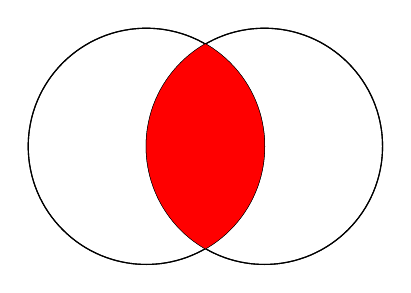
\begin{tikzpicture}
    \draw (-0.5,0) circle (1.5cm);
    \draw[black] (-0.5,0) circle (1.5cm);
    
    \draw (1,0) circle (1.5cm);
    \draw[black] (1,0) circle (1.5cm);
   \begin{scope}
        \clip (-0.5,0) circle (1.5cm);  
        \fill[red] (1,0) circle (1.5cm);  
    \end{scope} 
\end{tikzpicture}
\end{center}
\textbf{\underline{Left Join}}
A Left Join returns all rows from the left table and the matched rows from the right table. If there’s no match,
NULL values are returned for columns from the right table.

\begin{center}
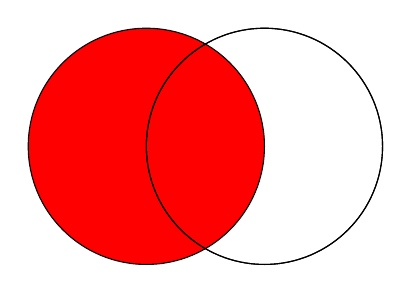
\begin{tikzpicture}
    \fill[red] (-0.5,0) circle (1.5cm);
    \draw[black] (-0.5,0) circle (1.5cm);

    \draw (1,0) circle (1.5cm);
    \draw[black] (1,0) circle (1.5cm);
\end{tikzpicture}
\end{center}
\textbf{\underline{Right Join}}
A Right Join returns all rows from the right table and the matched rows from the left table. If there’s no match,
NULL values are returned for columns from the left table.
\begin{center}
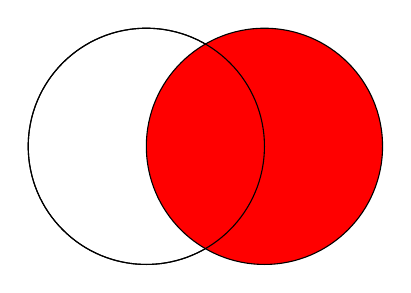
\begin{tikzpicture}
    \draw (-0.5,0) circle (1.5cm);

    \fill[red] (1,0) circle (1.5cm);

    \draw[black] (1,0) circle (1.5cm);
    \draw[black] (-0.5,0) circle (1.5cm);
\end{tikzpicture}
\end{center}
\textbf{\underline{Full Join}}
A Full Join returns all rows when there is a match in either left or right table. If there is no match,
NULL values are returned for unmatched columns.
\begin{center}
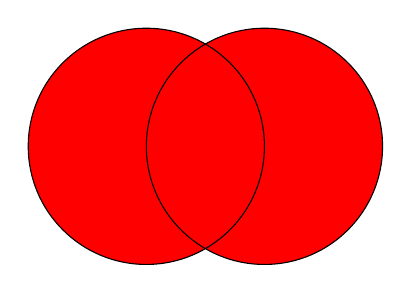
\begin{tikzpicture}
    \fill[red] (-0.5,0) circle (1.5cm);

    \fill[red] (1,0) circle (1.5cm);
    \draw[black] (1,0) circle (1.5cm);

    \draw[black] (-0.5,0) circle (1.5cm);
\end{tikzpicture}
\end{center}
\end{tcolorbox}

\subsubsection*{ \textbf{Syntax}}
\begin{tcolorbox}[title =Joins]
 \textbf{Inner Join}\\
\textcolor{blue}{SELECT} column$_{1}$,...,column$_{n}$ \textcolor{blue}{FROM} table1 \textcolor{blue}{INNER JOIN} 
table2 \textcolor{blue}{ON} table1.common\_column = table2.common\_column;

 \textbf{Left Join}\\
\textcolor{blue}{SELECT} column$_{1}$,...,column$_{n}$ \textcolor{blue}{FROM} table1 \textcolor{blue}{LEFT JOIN} 
table2 \textcolor{blue}{ON} table1.common\_column = table2.common\_column;

\textbf{Right Join}\\
\textcolor{blue}{SELECT} column$_{1}$,...,column$_{n}$ \textcolor{blue}{FROM} table1 \textcolor{blue}{RIGHT JOIN} 
table2 \textcolor{blue}{ON} table1.common\_column = table2.common\_column;

\textbf{Full Join}\\
\textcolor{blue}{SELECT} column$_{1}$,...,column$_{n}$ \textcolor{blue}{FROM} table1 \textcolor{blue}{FULL OUTER JOIN} 
table2 \textcolor{blue}{ON} table1.common\_column = table2.common\_column;
\end{tcolorbox}

 \subsection{Aggregation Functions}
\begin{tcolorbox}[title = Definition]
   Aggregation functions perform calculations on a set of values and return a single result. They are commonly used in conjunction with the \textcolor{blue}{GROUP BY} clause to summarize data.
   \begin{itemize}
    \item \textbf{Avg()} : Calculates the average (mean) of numeric values in a specified column.
    \item \textbf{Min()} : Returns the smallest (minimum) value in a specified column.
    \item \textbf{Max()} : Returns the largest (maximum) value in a specified column.
    \item \textbf{Count()} : Counts the number of non-null entries in a specified column (or all rows if * is used).
      \begin{itemize}
        \item  \textbf{count(*)} : Counts All rows
        \item  \textbf{count(column$_{i}$)} : counts number of rows where column$_{i}$ is not null
        \item  \textbf{count(distinct column$_{i}$)} : counts number of rows where column$_{i}$ is not null without repetition
    \end{itemize}
    \item \textbf{Sum()} : Adds up all values in a specified numeric column.
   \end{itemize} 
\end{tcolorbox}


\subsection{Operators}
\begin{tcolorbox}[title = Definition]
Operators are symbols that specify operations to be performed on operands. They can be categorized as follows:
\begin{itemize}
    \item \textbf{Logical Operators}: Used to combine conditions.
          \begin{itemize} 
              \item Logical And : AND 
              \item Logical Or : OR 
              \item Logical Not : NOT 
              \end{itemize} 
    
    \item \textbf{Comparison Operators}: Used to compare values.
    \begin{itemize}
             \item Equal : = 
             \item Not Equal : != 
             \item Greater : \textgreater
             \item Greater Or Equal : \textgreater= 
             \item Less : \textless
             \item Less Or Equal : \textless= 
             \item Between : BETWEEN value$_{1}$ AND value$_{2}$
             \item In : IN (set of values)
             \end{itemize} 

    \item \textbf{Arithmetic Operators}: Used for mathematical calculations.
    \begin{itemize} 
           \item Multiplication : *
           \item Division : / 
           \item Sum : + 
           \item Subtraction : -
           \end{itemize}
   \end{itemize}
\end{tcolorbox}


\section{DML Commands}

\subsection{Insert}

\begin{tcolorbox}
To insert rows into a table, we use the \textcolor{blue}{INSERT} command. We can insert one row at a time or multiple rows at once from the same or different tables using the \textcolor{blue}{ALL} keyword.
\end{tcolorbox}

\subsubsection*{\underline{\textbf{Syntax}}}
\begin{tcolorbox}[title = Insert]
\textbf{Insert One Row At A Time}\\
\textcolor{blue}{INSERT INTO} tableName (column$_{1}$,...,column$_{n}$) \textcolor{blue}{VALUES} (value$_{1}$,...,value$_{n}$);

\textbf{Insert Multiple Rows}\\
\textcolor{blue}{INSERT ALL}\\
\textcolor{blue}{INTO} tableName$_{1}$ (column$_{1}$,...,column$_{n}$) \textcolor{blue}{VALUES} (value$_{1}$,...,value$_{n}$);\\
\textcolor{blue}{INTO} tableName$_{2}$ (column$_{1}$,...,column$_{n}$) \textcolor{blue}{VALUES} (value$_{1}$,...,value$_{n}$);\\
...........................................................................\\
\textcolor{blue}{INTO} tableName$_{n}$ (column$_{1}$,...,column$_{n}$) \textcolor{blue}{VALUES} (value$_{1}$,...,value$_{n}$);\\
\textcolor{blue}{SELECT} * \textcolor{blue}{FROM} dual;
\end{tcolorbox}

\subsection{Update}
\begin{tcolorbox}[title = Definition]
To change the values of some rows in a table, we use the \textcolor{blue}{UPDATE} command, accompanied by the \textcolor{blue}{WHERE} clause to update only specific rows.
\end{tcolorbox}

\subsubsection*{\underline{\textbf{Syntax}}}
\begin{tcolorbox}[title = Update]
\textcolor{blue}{UPDATE} tableName \textcolor{blue}{SET} column$_{1}$ = value$_{1}$,...,column$_{n}$ = value$_{n}$\\
\textcolor{blue}{WHERE} {[condition]};
\end{tcolorbox}

\subsection{Delete} 
\begin{tcolorbox}[title = Definition]
To delete rows from a table, we use the \textcolor{blue}{DELETE} command, accompanied by the \textcolor{blue}{WHERE} clause to delete specific rows. Although it is possible to delete all rows using \textcolor{blue}{DELETE}, it is better to use \textcolor{blue}{TRUNCATE} for that purpose due to performance considerations.
\end{tcolorbox}

\subsubsection*{\underline{\textbf{Syntax}}}
\begin{tcolorbox}[title = Delete]
\textbf{DELETE SPECIFIC ROWS}\\
\textcolor{blue}{DELETE FROM} tableName \textcolor{blue}{WHERE} {[condition]};

\textbf{DELETE ALL ROWS}\\
\textcolor{blue}{DELETE FROM} tableName;
\end{tcolorbox}



\section{PL/SQL}
\subsection{Introduction}

\begin{prettyBox}{What's PL/SQL ?}{myblue}
PL/SQL, or Procedural Language/Structured Query Language, is an extension of SQL. While SQL (Structured Query Language) is primarily used for CRUD operations (querying, inserting, updating, and deleting data in relational databases), PL/SQL allows for full programmatic control with features such as control structures (loops and conditionals), variables, and error handling with exceptions. This enables the creation of scripts that can automate tasks with functions, procedures, and triggers, implement complex business logic, and manipulate data at a higher level than SQL alone.
\end{prettyBox}

\vspace{0.25cm}

\begin{prettyBox}{Differences Between PL/SQL and SQL}{myblue}
\begin{itemize}
    \item SQL is limited to CRUD operations; PL/SQL adds procedural programming capabilities.
    \item PL/SQL provides advanced error handling through exceptions.
    \item PL/SQL supports modular programming with functions, procedures, and triggers.
    \item PL/SQL is specific to Oracle databases, whereas SQL is standardized across various databases.
\end{itemize} 
\end{prettyBox}

\vspace{0.5cm}

\subsection{Overview Of Plsql's Structure}

\begin{prettyBox}{Programme Structure}{myblue}
A PL/SQL has 3 blocks :
\begin{itemize}
    \item \textbf{DECLARE}(Optional Block) : contains all the declared variables , constants \& modules(functions,procedure) 
    \item \textbf{MAIN} : contains the main executable code 
    \item \textbf{EXCEPTION}(Optional Block) : handls erros with exceptions 
\end{itemize}
\end{prettyBox}

\begin{center}
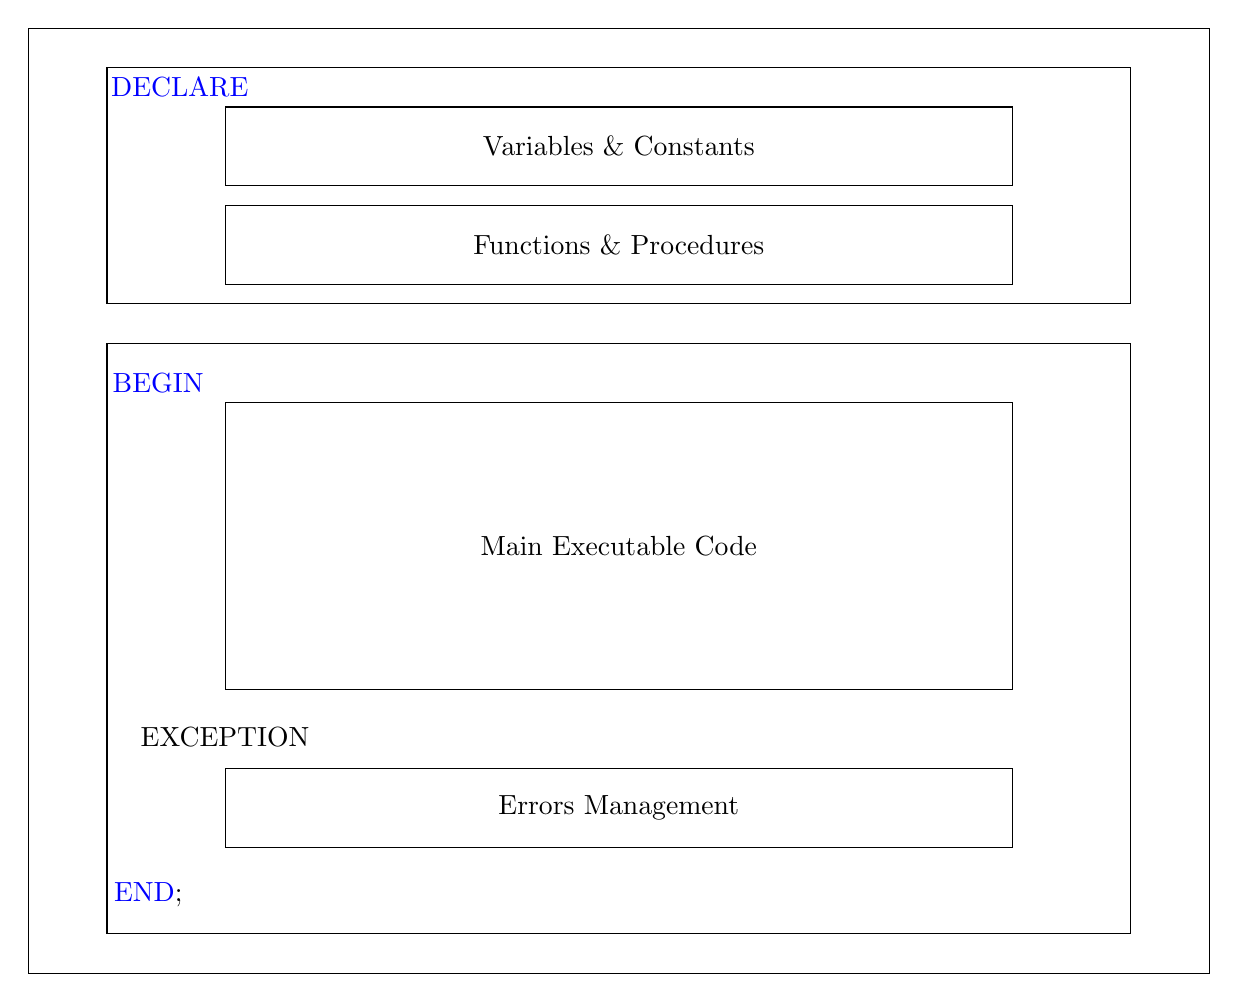
\begin{tikzpicture}
    \draw (0,0) rectangle (15,12);
    
    \draw (1,8.5) rectangle(14,11.5);
    \node at (1.925,11.25) {\textcolor{blue}{DECLARE}};
    \draw (2.5,10) rectangle (12.5,11);
    \node at(7.5,10.5){Variables \& Constants};
    \draw (2.5,8.75) rectangle (12.5,9.75);
    \node at (7.5,9.25){Functions \& Procedures};
    
    \draw (1,0.5) rectangle(14,8);
    \node at (1.65,7.5) {\textcolor{blue}{BEGIN}};
    \draw (2.5,3.6) rectangle (12.5,7.25);
    \node at (7.5,5.425){Main Executable Code};
    \node at (2.5,3) {EXCEPTION};
    \draw (2.5,1.6) rectangle (12.5,2.6);
    \node at (7.5,2.1){Errors Management};
    \node at (1.525,1) {\textcolor{blue}{END};};
\end{tikzpicture}
\end{center}

\vspace{0.5cm}

\subsection{Comments}


\subsubsection*{\underline{Syntax}}

\vspace{0.25cm}

\subsubsection*{\underline{Single Comment}}
\lstinputlisting{SQL/syntax/Pl_Sql/singleComment.sql}


\subsubsection*{\underline{Multi-Line Comment}}
\lstinputlisting{SQL/syntax/Pl_Sql/multiComment.sql}


\vspace{0.5cm}


\subsection{Printing}

\begin{prettyBox}{DBMS\_OUTPUT.PUT\_LINE}{myblue}
To print messages in the console, we use the \texttt{DBMS\_OUTPUT.PUT\_LINE} command. The message should be enclosed
in single quotes ' ' and we use double pipes \texttt{||} to concatenate with variables.
\end{prettyBox}

\subsubsection*{\underline{Syntax}}


\lstinputlisting{SQL/syntax/Pl_Sql/print.sql}

\vspace{0.25cm}

\begin{prettyBox}{Note}{red}
To be able to see the printed messages in the console of SQL*Plus, SQL Developer, ...etc, we need to activate
the buffer responsible for printing the messages by using the command: 

\lstinputlisting{SQL/syntax/Pl_Sql/server.sql}

Note that this is only needed once , and it will remain active unless you explicitly turn it off.
\end{prettyBox}

\vspace{0.5cm}

\subsection{Variables Declaration \& Types}

\begin{prettyBox}{Variables \& Constants}{myblue}
All variables and constants must be declared in the \textcolor{blue}{DECLARE} scope , 
we use := to affect values to variables 
\end{prettyBox}

\subsubsection*{\underline{Syntax}}

\lstinputlisting{SQL/syntax/Pl_Sql/varDeclaration.sql}

\vspace{0.25cm}
\begin{prettyBox}{Types}{myblue}
PL/SQL supports all data types normal sql has like those we've seen previously. Here, we introduce two additional types:

\begin{itemize}
    \item \textbf{Type:} Used to define a variable with the same data type as a column in a table:
    
\lstinputlisting{SQL/syntax/Pl_Sql/type.sql}

    \item \textbf{RowType:} Used to define a variable as a record with the structure of a row in a table:
\lstinputlisting{SQL/syntax/Pl_Sql/rowType.sql}
\end{itemize}

\end{prettyBox}



\begin{prettyBox}{Store Select Output In Variables}{myblue}
We can store the output of the \textcolor{blue}{SELECT} command in variables using the \textcolor{blue}{INTO} clause as follows:
\end{prettyBox}

\subsubsection*{\underline{Syntax}}

\lstinputlisting{SQL/syntax/Pl_Sql/select.sql}

\vspace{0.25cm}

\begin{prettyBox}{Note}{red}
\textbf{\underline{Order Of Variables Is Important}}

\vspace{0.15cm}
The order of the variables in the \textcolor{blue}{INTO} clause must match the order of the selected columns

\vspace{0.25cm}
\textbf{\underline{Select Should Ouput One Line Only}}

\vspace{0.15cm}
When Storing the output of \textcolor{blue}{SELECT} in variables , the ouput should be one line and not a table
if not we will have to use cursor to navigate through the table we will cover that later on


\vspace{0.25cm}

\textbf{\underline{We Must Use Store Select Output}}

\vspace{0.15cm}
In PL/SQL we have to always store the output of a select if not we will have a complilation error
\end{prettyBox}

\vspace{0.5cm}
\subsection{Control Structures}

\begin{prettyBox}{Definition}{myblue}
In PL/SQL, control structures are constructs that help control the flow of execution in a block of code.
They determine the order and conditions under which statements are executed and help make the code dynamic
and responsive to varying conditions. The main types of control structures in PL/SQL are:
\end{prettyBox}

\vspace{0.25cm}

\subsubsection{Conditional Control}
\newpage
\subsubsection*{\underline{If}} 
\subsubsection*{\underline{Syntax}}

\lstinputlisting{SQL/syntax/Pl_Sql/if.sql}


\vspace{0.25cm}

\subsubsection*{\underline{Switch Case}}

\subsubsection*{\underline{Syntax}}

\lstinputlisting{SQL/syntax/Pl_Sql/case.sql}

\vspace{0.25cm}

\subsubsection{Looping Control}

\subsubsection*{\underline{Simple Loop}}


\subsubsection*{\underline{Syntax}}


\lstinputlisting{SQL/syntax/Pl_Sql/simpleLoop.sql}



\subsubsection*{\underline{While Loop}}

\subsubsection*{\underline{Syntax}}


\lstinputlisting{SQL/syntax/Pl_Sql/whileLoop.sql}


\vspace{0.25cm}



\subsubsection*{\underline{For Loop}}

\subsubsection*{\underline{Syntax}}


\lstinputlisting{SQL/syntax/Pl_Sql/forLoop.sql}

\vspace{0.5cm}

\subsection{Raise Application Error}
\begin{prettyBox}{Raise Errors}{myblue}
RAISE\_APPLICATION\_ERROR is a procedure used to raise an error that halts code execution, with a custom error
message. Each error\_code (between -20000 and -20999) is associated with an error message retrieved 
by SQLERRM, while SQLCODE captures the error code itself.

\vspace{0.25cm}


\lstinputlisting{SQL/syntax/Pl_Sql/raise_application.sql}

\vspace{0.25cm}


Though commonly used to handle user-defined exceptions, RAISE\_APPLICATION\_ERROR can also be used internally
by the system for predefined exceptions, supporting error control in both system and custom PL/SQL operations.
\end{prettyBox}


\subsection{Exceptions}
\begin{prettyBox}{Exception}{myblue}
Exceptions help manage errors . Under
the hood, exceptions are built on RAISE\_APPLICATION\_ERROR ,  only difference is that it's more readable. There are two main types of exceptions:
\begin{itemize}
    \item \textbf{Predefined Exceptions}: These are system-defined exceptions, such as:
        \begin{itemize}
            \item NO\_DATA\_FOUND: Raised when a \textcolor{blue}{SELECT} statement returns no rows.
            \item TOO\_MANY\_ROWS: Raised when a \textcolor{blue}{SELECT} statement returns more than one row.
        \end{itemize}
    \item \textbf{User-defined Exceptions}: Defined by the user using the \textcolor{blue}{EXCEPTION} DataType.
\end{itemize}
\end{prettyBox}

\subsubsection*{\underline{Syntax}}


\lstinputlisting{SQL/syntax/Pl_Sql/exc.sql}




\begin{tcolorbox}[title = Exceptions with SQLCODE]
    
    \textcolor{blue}{DECLARE}

     sqlcode\_1 := -20001;
    
     sqlcode\_2 := -20002;

     \textcolor{blue}{BEGIN}
    
     \textcolor{commentgray}{- - Check for specific conditions and raise custom errors with codes}
   
    IF [Condition] \textcolor{blue}{THEN}
    
    RAISE\_APPLICATION\_ERROR(sqlcode\_1, \textcolor{messagegreen}{'error message1'});
    
    [Condition] \textcolor{blue}{THEN}
    
    RAISE\_APPLICATION\_ERROR(sqlcode\_2, \textcolor{messagegreen}{'error message2'});
    
    \textcolor{blue}{END} IF;

EXCEPTION

\textcolor{blue}{WHEN} OTHERS \textcolor{blue}{THEN}

\textcolor{commentgray}{- - Use SQLCODE to check error codes directly}

IF SQLCODE = sqlcode\_1 \textcolor{blue}{THEN}

DBMS\_OUTPUT.PUT\_LINE(\textcolor{messagegreen}{'Error: '} \texttt{||} SQLERRM);

ELSIF SQLCODE = sqlcode\_2 \textcolor{blue}{THEN}

DBMS\_OUTPUT.PUT\_LINE(\textcolor{messagegreen}{'Error: '} \texttt{||} SQLERRM);

\textcolor{blue}{ELSE}

DBMS\_OUTPUT.PUT\_LINE(\textcolor{messagegreen}{'Unexpected error: '} \texttt{||} SQLERRM);

\textcolor{blue}{END} IF;

\textcolor{blue}{END};

\end{tcolorbox}

\begin{prettyBox}{Note}{red}
\textbf{What is OTHERS?}

It’s best practice to add OTHERS as the last exception handler, as it catches any exceptions not explicitly
defined. This ensures any unexpected errors are managed gracefully.

\textbf{When to Use RAISE\_APPLICATION\_ERROR vs. Exceptions?}

Although exceptions are built on RAISE\_APPLICATION\_ERROR, they offer better readability and manageability
in complex code. Use exceptions for organized error handling, while RAISE\_APPLICATION\_ERROR provides a more
direct and minimalistic approach.
\end{prettyBox}

\vspace{0.5cm}

\subsection{Cursors}
\begin{tcolorbox}[title = cursor]
    \begin{verbatim}
DECLARE
    -- Declare a cursor that selects data
    CURSOR cr IS
        select query

    -- Variables to hold fetched data
    var1 table.col1%TYPE;
    var2 table.col2%TYPE;
    .....
    varn table.coln%TYPE;
BEGIN
    -- Open the cursor
    OPEN emp_cursor;
    FETCH cr INTO var1,var2,...,varn
    -- Loop through the result set
    WHILE(cr%FOUND) LOOP
        --traitements
        FETCH cr INTO var1,var2,...,varn
        
    END LOOP;

    -- Close the cursor
    CLOSE emp_cursor;
END;
    \end{verbatim}
\end{tcolorbox}
\subsection{Triggers}
\subsection{Functions}
\subsection{Procedure}


\end{document}

%only able to do out of line with constraint : fix example , syntax and some box

